\usetikzlibrary{calc,arrows.meta,patterns,angles,quotes}
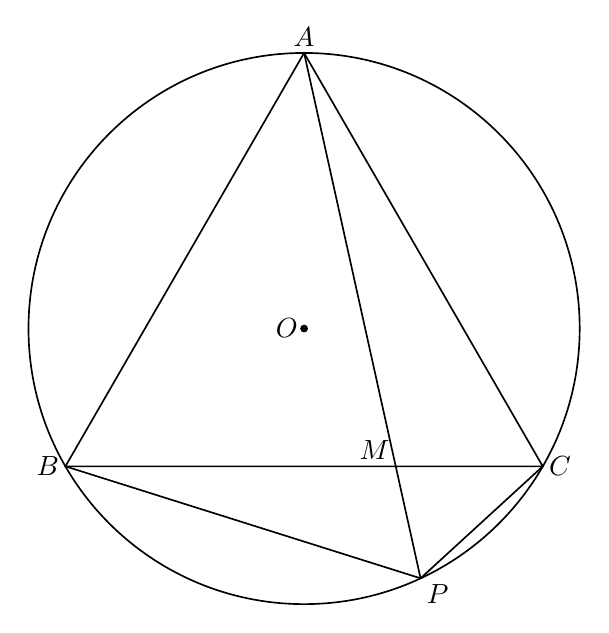
\begin{tikzpicture}[x=1cm,y=1cm,line width=.6pt,font=\normalsize,>=Stealth]
\coordinate (O) at (0.0000000000,0.0000000000);
\coordinate (A) at (0.0000000000,3.5000000000);
\coordinate (B) at (-3.0310889132,-1.7500000000);
\coordinate (C) at (3.0310889132,-1.7500000000);
\coordinate (P) at (1.4791639161,-3.1720772546);
\coordinate (M) at (1.1638969789,-1.7500000000);
\draw (O) circle[radius=3.5000000000cm];
\draw (A)--(B)--(C)--(A);
\draw (A)--(P);
\draw (B)--(P);
\draw (P)--(C);
\fill (O) circle[radius=1.4pt];
\node[above=2pt,inner sep=0pt] at (A) {$A$};
\node[left=2pt,inner sep=0pt] at (B) {$B$};
\node[right=2pt,inner sep=0pt] at (C) {$C$};
\node[below right=2pt,inner sep=0pt] at (P) {$P$};
\node[above left=2pt,inner sep=0pt] at (M) {$M$};
\node[left=2pt,inner sep=0pt] at (O) {$O$};
\end{tikzpicture}
